\documentclass[11pt,a4paper,oldfontcommands]{memoir}
\usepackage{ctex}
\usepackage[utf8]{inputenc}
\usepackage[T1]{fontenc}
\usepackage{microtype}
\usepackage[dvips]{graphicx}
\usepackage{xcolor}
\usepackage{times}
\usepackage{listings}
\usepackage{courier}
\lstset{
    columns=fixed,       
    numbers=left,                                        % 在左侧显示行号
    frame=none,                                          % 不显示背景边框
    backgroundcolor=\color[RGB]{245,245,244},            % 设定背景颜色
    keywordstyle=\color[RGB]{40,40,255},                 % 设定关键字颜色
    numberstyle=\footnotesize\color{darkgray},           % 设定行号格式
    commentstyle=\color[RGB]{0,96,96},                % 设置代码注释的格式
    stringstyle=\rmfamily\slshape\color[RGB]{128,0,0},   % 设置字符串格式
    showstringspaces=false,                              % 不显示字符串中的空格
    language=c++,                                        % 设置语言
    basicstyle=\small\ttfamily
}

\usepackage[
breaklinks=true,colorlinks=true,
%linkcolor=blue,urlcolor=blue,citecolor=blue,% PDF VIEW
linkcolor=black,urlcolor=black,citecolor=black,% PRINT
bookmarks=true,bookmarksopenlevel=2]{hyperref}

\usepackage{amsmath}

\usepackage{geometry}
% PDF VIEW
% \geometry{total={210mm,297mm},
% left=25mm,right=25mm,%
% bindingoffset=0mm, top=25mm,bottom=25mm}
% PRINT
\geometry{total={210mm,297mm},
left=20mm,right=20mm,
bindingoffset=10mm, top=25mm,bottom=25mm}

\OnehalfSpacing
\chapterstyle{bianchi}
\setsecheadstyle{\Large\bfseries\sffamily\raggedright}
\setsubsecheadstyle{\large\bfseries\sffamily\raggedright}
\setsubsubsecheadstyle{\bfseries\sffamily\raggedright}

\pagestyle{plain}
\makepagestyle{plain}
\makeevenfoot{plain}{\thepage}{}{}
\makeoddfoot{plain}{}{}{\thepage}
\makeevenhead{plain}{}{}{}
\makeoddhead{plain}{}{}{}
\maxsecnumdepth{subsection} % chapters, sections, and subsections are numbered
\maxtocdepth{subsection} % chapters, sections, and subsections are in the Table of Contents

\graphicspath{ {./figure/} }
\begin{document}
\thispagestyle{empty}
{
\sffamily
\centering
{\LARGE
Introduction To 3D Game Programming with DirectX12 笔记
}

\vspace{3.5cm}
(草稿)
\clearpage
\tableofcontents*
\clearpage
\chapter{向量代数(Vector Algebra)}
\chapter{矩阵代数(Matrix Algebra)}
\chapter{矩阵变换(Transformation)}
\chapter{Direct3D 初始化(Direct3D Initialization)}

\chapter{渲染管道(The Rendering Pipeline)}
\section{3D图像(The 3D Illusion)}
\section{模型表达(Model Representation)}
\section{基本计算颜色(Basic Computer Color)}
\begin{flushleft}
计算机显示器在每个像素发射一种混合红、绿、蓝三种颜色的光。当这种混合光到达眼睛并且击中视网膜区域,视锥细胞收到刺激并将产生的神经冲动通过视觉神经传递到大脑。大脑解释这种信号为颜色。随着混合光的变化,使这些视锥细胞收到不同的刺激,从而使大脑中产生不同的颜色。
\end{flushleft}

\subsection{颜色运算(Color Operations)}
\begin{itemize}
    \item 加法:$(0.0, 0.5, 0) + (0, 0.0, 0.25) = (0.0, 0.5, 0.25)$
    \item 减法:$(1, 1, 1) - (1, 1, 0) = (0, 0, 1)$
    \item 标量乘法:$0.5(1, 1, 1) = (0.5, 0.5, 0.5)$
    \item 显然,点乘和叉乘对于颜色向量来说没有意义。然而,颜色向量有一特殊的运算称为调制或分量乘法:$(c_{r},c_{g},c_{b}) \otimes (k_{r},k_{g},k_{b}) = (c_{r}k_{r},c_{g}k_{g},c_{b}k_{b})$。该运算主要用来作为照明方程。举个例子,假设我们有一束入射光线(r,g,b),它会照射一个反射50%红光,75%绿光和25%蓝光的表面,并吸收剩余的光线。 然后反射光线的颜色由下式给出:$(r,g,b) \otimes (0.5,0.75,0.25) = (0.5r,0.75g,0.25b)$
\end{itemize}

\subsection{128位颜色(128-Bit Color)}
\begin{flushleft}
通常我们会合并另外的颜色分量,称作 alpha 分量。alpha 分量常用来表示颜色的透明度(透明度在混合中很有用,因为我们还没有使用混合,目前只需将 alpha 分量设为 1 即可)。包含 alpha 分量意味着我们用 4D 颜色向量$(r, g, b, a), 0 \leq r,g,b,a \leq 1$ 为了用 128-bits 表示一种颜色,每个分量使用浮点型值。因为数学上,一种颜色就是一个 4D 向量,我们能在代码中使用 XMVECTOR 类型来表示一种颜色,并且每当调用 DirectX Math 中的向量函数时都会受益于 SIMD (如,颜色加减和标量乘法)。为了方便分量乘法,DirectX Math 库提供了下面方法:
\begin{lstlisting}
// Return c1 \otimes c2
XMVECTOR XM_CALLCONV XMColorModulate(FXMVECTOR C1, FXMVECTOR C2);
\end{lstlisting}
\end{flushleft}

\subsection{32位颜色(32-Bit Color)}
\begin{flushleft}
要以32位大小来表示一个颜色,可以给每个分量分配一个字节(8-bit)大小。这样一来,每个分量最多能表现256种色调——0代表无强度,255代表满强度,中间值代表中间强度。看似每个分量一个字节很小,但是组合在一起$(256 \times 256 \times 256)$就表示百万种不同的颜色。DirectX Math 库(\#include <DirectXPackedVector.h>) DirectX::PackedVector 命名空间(namespace)下提供了以下数据结构来存储32位颜色:
\begin{lstlisting}
namespace DirectX
{
namespace PackedVector
{
    // ARGB Color; 8-8-8-8 bit unsigned normalized integer components packed
    // into a 32 bit integer. The normalized color is packed into 32 bits
    // using 8 bit unsigned, normalized integers for the alpha, red, green,
    // and blue components.
    // The alpha component is stored in the most significant bits and the
    // blue component in the least significant bits (A8R8G8B8):
    // [32] aaaaaaaa rrrrrrrr gggggggg bbbbbbbb [0]
    struct XMCOLOR
    {
        union
        {
            struct
            {
                uint8_t b; // Blue: 0/255 to 255/255
                uint8_t g; // Green: 0/255 to 255/255
                uint8_t r; // Red: 0/255 to 255/255
                uint8_t a; // Alpha: 0/255 to 255/255
            };
            uint32_t c;
        };
        XMCOLOR() {}
        XMCOLOR(uint32_t Color) : c(Color) {}
        XMCOLOR(float _r, float _g, float _b, float _a);
        explicit XMCOLOR(_In_reads_(4) const float *pArray);
        operator uint32_t () const { return c; }
        XMCOLOR& operator= (const XMCOLOR& Color) 
        { c = Color.c; return *this; }
        XMCOLOR& operator= (const uint32_t Color) 
        { c = Color; return *this; }
    };
} // end PackedVector namespace
} // end DirectX namespace
\end{lstlisting}
一个32位颜色数据能被转换为128位颜色数据: 将整数区间$[0, 255]$ 映射到实数区间$[0, 1]$。每个数除以255即可,也就是说 设$0 \leq n \leq 255$,且 n 是整数,则 $0 \leq \frac{n}{255} \leq 1$ 就是需要的范围 0 到 1 的颜色强度。例:(80,140,200,255)转换如下:
$$ (80,140,200,255)\rightarrow (\frac{80}{255},\frac{140}{255},\frac{200}{255},\frac{255}{255}) \approx (0.31,0.55,0.78,1.0)$$
另一方面,128位颜色能转换为32位颜色:将每个分量乘以255并且四舍五入取整。例:
$$(0.3,0.6,0.9,1.0)\rightarrow (0.3\cdot 255,0.6\cdot 255,0.9\cdot 255,1.0\cdot 255)=(77,153,230,255)$$

在将32位颜色转换为128位颜色时通常必须执行额外的位操作,反之,因为8位颜色组件通常打包为32位整数值(如 unsigned int),XMCOLOR 就是如此。DirectXMath 库定义了一个方法以 XMCOLOR 作为参数,返回XMVECTOR:
\begin{lstlisting}
XMVECTOR XM_CALLCONV PackedVector::XMLoadColor(const XMCOLOR* pSource);
\end{lstlisting}
\end{flushleft}

\subsection{渲染管道概览(Overview of the rendering pipeline)}
\subsection{输入汇编程序阶段(The Input Assembler Stage)}
\subsubsection{顶点(Vertices)}
\subsubsection{原始拓扑(Primitive Topology)}
\subsubsection{指数(Indices)}
\subsection{顶点着色器阶段(The Vertex Shader Stage)}
\subsubsection{本地空间和世界空间(Local Space and World Space)}
\subsubsection{视图空间(View Space)}
\begin{flushleft}
为了形成场景的二维图像,我们必须在场景中放置一个虚拟相机。 相机指定了观众可以看到的世界的多大的体积,以及我们需要生成多大的世界体积来生成二维图像。让我们将一个局部坐标系统(称为视图空间,眼图空间或相机空间)附加到相机,如图\ref{fig:5-19}所示; 也就是说,摄像机坐落在正视z轴的原点处,x轴指向摄像机的右侧,y轴指向摄像机的上方。 而不是描述相对于世界空间的场景顶点,基于相机坐标系,渲染管线的后面阶段很方便地描述它们。从世界空间到视图空间的坐标变换称为视图变换,相应的矩阵称为视图矩阵。\\
\begin{figure}[t]
    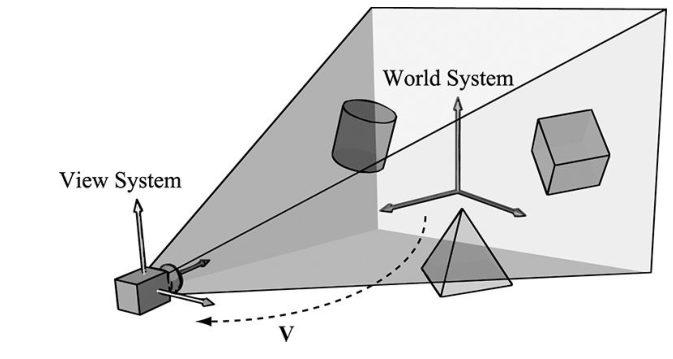
\includegraphics[width=\textwidth]{5-19}
    \centering
    \caption{转换顶点相对于世界空间的坐标,使它们相对于相机空间。}
    \label{fig:5-19}
\end{figure}
如果$Q_{w}=(Q_{x},Q_{y},Q_{z},1)$,$u_{w}=(u_{x},u_{y},u_{z},0)$,$v_{w}=(v_{x},v_{y},v_{z},0)$,$w_{w}=(w_{x},w_{y},w_{z},0)$分别用相对于世界空间的齐次坐标来描述视图空间的原点,x轴,y轴和z轴,然后我们从§3.4.3知道坐标矩阵从视图空间的变化到世界空间是:
$$W=
\begin{bmatrix}
u_{x} & u_{y} & u_{z} & 0\\
v_{x} & v_{y} & v_{z} & 0\\
w_{x} & w_{y} & w_{z} & 0\\
Q_{x} & Q_{y} & Q_{z} & 1
\end{bmatrix}$$
\end{flushleft}
\end{document}

